\section{High-Level Architecture}
The system is designed around a decoupled Client-Server architecture, logically partitioned into three Maven modules:
\begin{itemize}
    \item \textbf{Backend:} Contains the server logic, built upon the Spring Boot framework.
    \item \textbf{Client:} Contains the consumer JavaFX desktop application.
    \item \textbf{Shared:} Contains standard enums, utilities and Data Transfer Objects (DTOs) common to both the server and the client. In addition to avoiding code repetition, this module guarantees both communication sides serialize and deserialize payloads using the exact same class definitions, ensuring strict network type-safety.
\end{itemize}

Such a structure ensures the backend remains entirely agnostic to the presentation layer, relying strictly on standard data-exchange formats (JSON) over the HTTP protocol.

\begin{figure}[H]
\centering
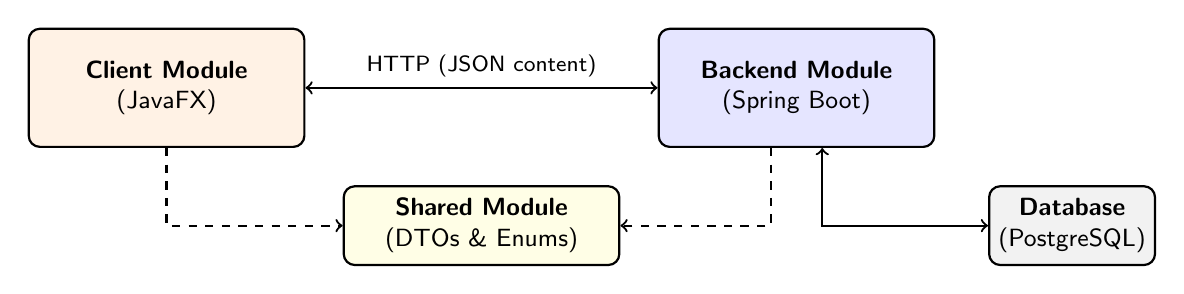
\begin{tikzpicture}[
    box/.style={draw=black, thick, rounded corners, minimum width=3.5cm, minimum height=1.5cm, align=center, fill=blue!5, font=\sffamily\small},
    dbbox/.style={draw=black, thick, rounded corners, minimum height=1.5cm, minimum width=2cm, fill=yellow!10, align=center, font=\sffamily\small},
    arrow/.style={->, thick},
    dasharrow/.style={->, dashed, thick}
]
    \node[box, fill=orange!10] (client) at (-4, 0) {\textbf{Client Module} \\ (JavaFX)};
    \node[box, fill=blue!10] (backend) at (4, 0) {\textbf{Backend Module} \\ (Spring Boot)};
    \node[box, minimum height=1cm, fill=yellow!10] (shared) at (0, -1.75) {\textbf{Shared Module} \\ (DTOs \& Enums)};
    \node[dbbox, minimum height=1cm, fill=gray!10] (db) at (7.5, -1.75) {\textbf{Database} \\ (PostgreSQL)};

    \draw[arrow, <->] (client) -- node[above, font=\footnotesize\sffamily] {HTTP (JSON content)} (backend);
    \draw[dasharrow] (client) |- (shared);
    \draw[dasharrow] ([xshift=-0.75cm] backend) |- (shared);
    \draw[arrow, <->] ([xshift=0.75cm] backend) |- (db);

\end{tikzpicture}
\caption{High-Level Modular Architecture}
\end{figure}

\section{Technological Stack}
The application leverages \textbf{Java 17+} and relies on the following core technologies to fulfill its functional and non-functional requirements:

\begin{itemize}
    \item \textbf{Server:} \textit{Spring Boot} provides the foundational inversion of control and auto-configuration. Routing is handled by \textit{Spring Web MVC}, while \textit{Spring Security} enforces JWT-based authentication. The data layer utilizes \textit{Spring Data JPA} and \textit{Hibernate} for Object-Relational Mapping (ORM) against a relational database (\textit{PostgreSQL} / \textit{H2} (for testing)).
    \item \textbf{Client:} \textit{JavaFX} serves as the framework for the Graphical User Interface.
    \item \textbf{Tooling:} \textit{Apache Maven} coordinates multi-module dependency management and the build lifecycle. \textit{JUnit 5} and \textit{Mockito} facilitate unit testing and test-driven development methodologies.
\end{itemize}

\section{Backend Architecture}
The server implements a strict 3-tier logical layered architecture, which separates concerns and isolates business logic from the network protocols.

\begin{enumerate}
    \item \textbf{Controller Layer:} Handles incoming HTTP connections, maps REST endpoints, and deserializes JSON requests. It delegates instructions to the underlying services, then serializes the results into a JSON response that gets sent back to the requesting client.
    \item \textbf{Service Layer:} This tier encapsulates the core business rules (e.g. debt reduction algorithms). It performs strict validation and defines transactional boundaries to guarantee data atomicity and avoid corruption.
    \item \textbf{Data Access Layer (Repository):} Contains Spring Data JPA interfaces that abstract raw SQL, handling complex queries that map database tables directly to standard Java Objects.
\end{enumerate}

\section{Client Architecture}
The client module implements an API-first architectural design. It mirrors the backend services via dedicated client-side classes injected with a centralized HTTP client wrapper. These classes build requests, include the session JWT in the \texttt{'Authorization: Bearer'} header and deserialize the JSON server responses. By wrapping the REST communication in these service classes, the JavaFX UI controllers remain completely unaware of the underlying network protocols, adhering strictly to the Single Responsibility Principle.

\section{Detailed Architecture Diagram}

\begin{figure}[H]
    \centering
    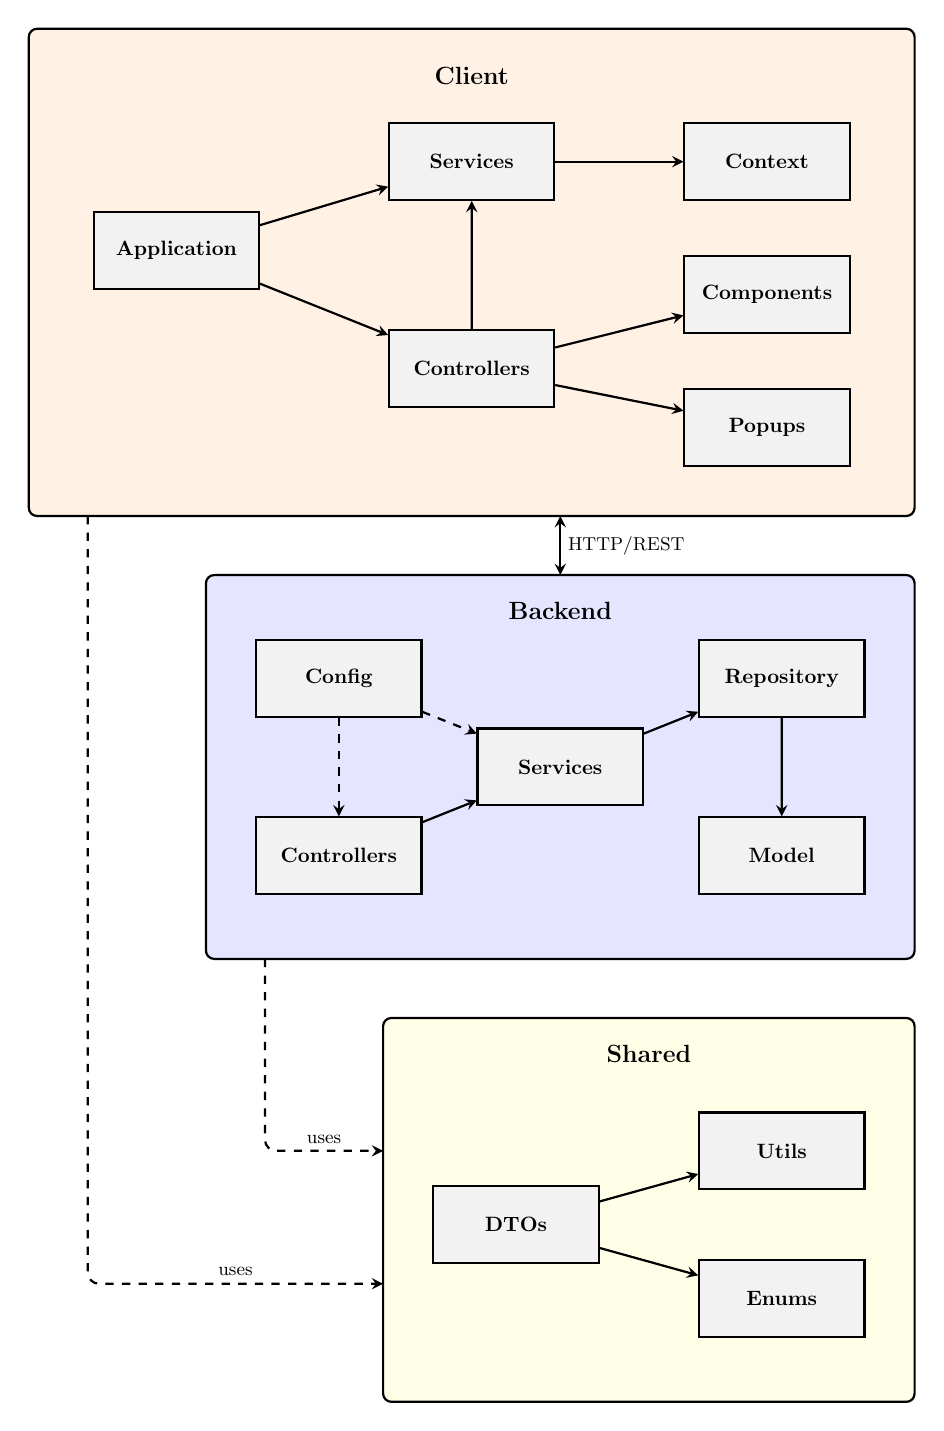
\begin{tikzpicture}[
        scale=0.75, transform shape, % <--- Adjust the 0.7 to change the overall size
        font=\sffamily,
        >=stealth,
        % Define the style for simple rectangles
        umlbox/.style={
            rectangle, draw, thick, fill=gray!10,
            minimum width=2.8cm, minimum height=1.3cm,
            align=center, font=\bfseries
        }
    ]
    
        % ==========================
        % BOUNDING BOXES (BACKGROUND)
        % ==========================
        % Client Box
        \draw[thick, fill=orange!10, rounded corners=3pt] (-5, 2.25) rectangle (10, -6);
        \node[font=\bfseries\large] at (2.5, 1.45) {\textbf{Client}};
    
        % Backend Box
        \draw[thick, fill=blue!10, rounded corners=3pt] (-2, -7) rectangle (10, -13.5);
        \node[font=\bfseries\large] at (4, -7.6) {\textbf{Backend}};
    
        % Shared Box
        \draw[thick, fill=yellow!10, rounded corners=3pt] (1, -14.5) rectangle (10, -21);
        \node[font=\bfseries\large] at (5.5, -15.1) {\textbf{Shared}};
    
    
        % ==========================
        % CLIENT NODES
        % ==========================
        % Neatly arranged in a 3-column grid within the client bounds
        \node[umlbox] (app)       at (-2.5, -1.5) {Application};
        \node[umlbox] (svcClient) at (2.5, 0)     {Services};
        \node[umlbox] (ctrl)      at (2.5, -3.5)    {Controllers};
        \node[umlbox] (ctx)       at (7.5, 0)     {Context};
        \node[umlbox] (comp)      at (7.5, -2.25)  {Components};
        \node[umlbox] (pop)       at (7.5, -4.5)  {Popups};
    
        % Client Connections
        \draw[->, thick] (app) -- (svcClient);
        \draw[->, thick] (app) -- (ctrl);
        \draw[->, thick] (ctrl) -- (svcClient);
        \draw[->, thick] (ctrl) -- (comp);
        \draw[->, thick] (ctrl) -- (pop);
        \draw[->, thick] (svcClient) -- (ctx);
    
    
        % ==========================
        % BACKEND NODES
        % ==========================
        % Arranged to flow from left to right within the backend bounds
        \node[umlbox] (config)      at (0.25, -8.75)  {Config};
        \node[umlbox] (ctrlBackend) at (0.25, -11.75) {Controllers};
        \node[umlbox] (svcBackend)  at (4, -10.25)   {Services};
        \node[umlbox] (repo)        at (7.75, -8.75)  {Repository};
        \node[umlbox] (model)       at (7.75, -11.75) {Model};
    
        % Backend Connections
        \draw[->, thick, dashed] (config) -- (svcBackend);
        \draw[->, thick, dashed] (config) -- (ctrlBackend);
        \draw[->, thick] (ctrlBackend) -- (svcBackend);
        \draw[->, thick] (svcBackend) -- (repo);
        \draw[->, thick] (repo) -- (model);
    
    
        % ==========================
        % SHARED NODES
        % ==========================
        % Centered hierarchically within the shared bounds
        \node[umlbox] (dto)   at (3.25, -18) {DTOs};
        \node[umlbox] (utils) at (7.75, -16.75)   {Utils};
        \node[umlbox] (enums) at (7.75, -19.25)   {Enums};
    
        % Shared Connections
        \draw[->, thick] (dto) -- (utils);
        \draw[->, thick] (dto) -- (enums);
    
    
        % ==========================
        % CROSS-BOUNDARY DEPENDENCIES
        % ==========================
        % Client -> Backend (HTTP/REST)
        \draw[<->, thick] (4, -6) -- 
            node[right, font=\small] {HTTP/REST} (4, -7);
    
        % Client -> Shared (uses)
        % Uses orthogonal routing ( |-) to bypass the backend box safely on the left
        \draw[->, thick, dashed, rounded corners] (-4, -6) |- 
            node[pos=0.75, above, font=\small] {uses} (1, -19);
    
        % Backend -> Shared (uses)
        \draw[->, thick, dashed, rounded corners] (-1, -13.5) |- 
            node[pos = 0.75, above, font=\small] {uses} (1, -16.75);
    
    \end{tikzpicture}
    \caption{Detailed architecture diagram}
    \label{fig:uml_overview}
\end{figure}

\section{Example: User Request Flow}

The following diagram illustrates the lifecycle of a user request, tracing its path through the architecture, its interaction with the database and the return of the response back to the user.

\begin{figure}[H]
\centering
\resizebox{\textwidth}{!}{%
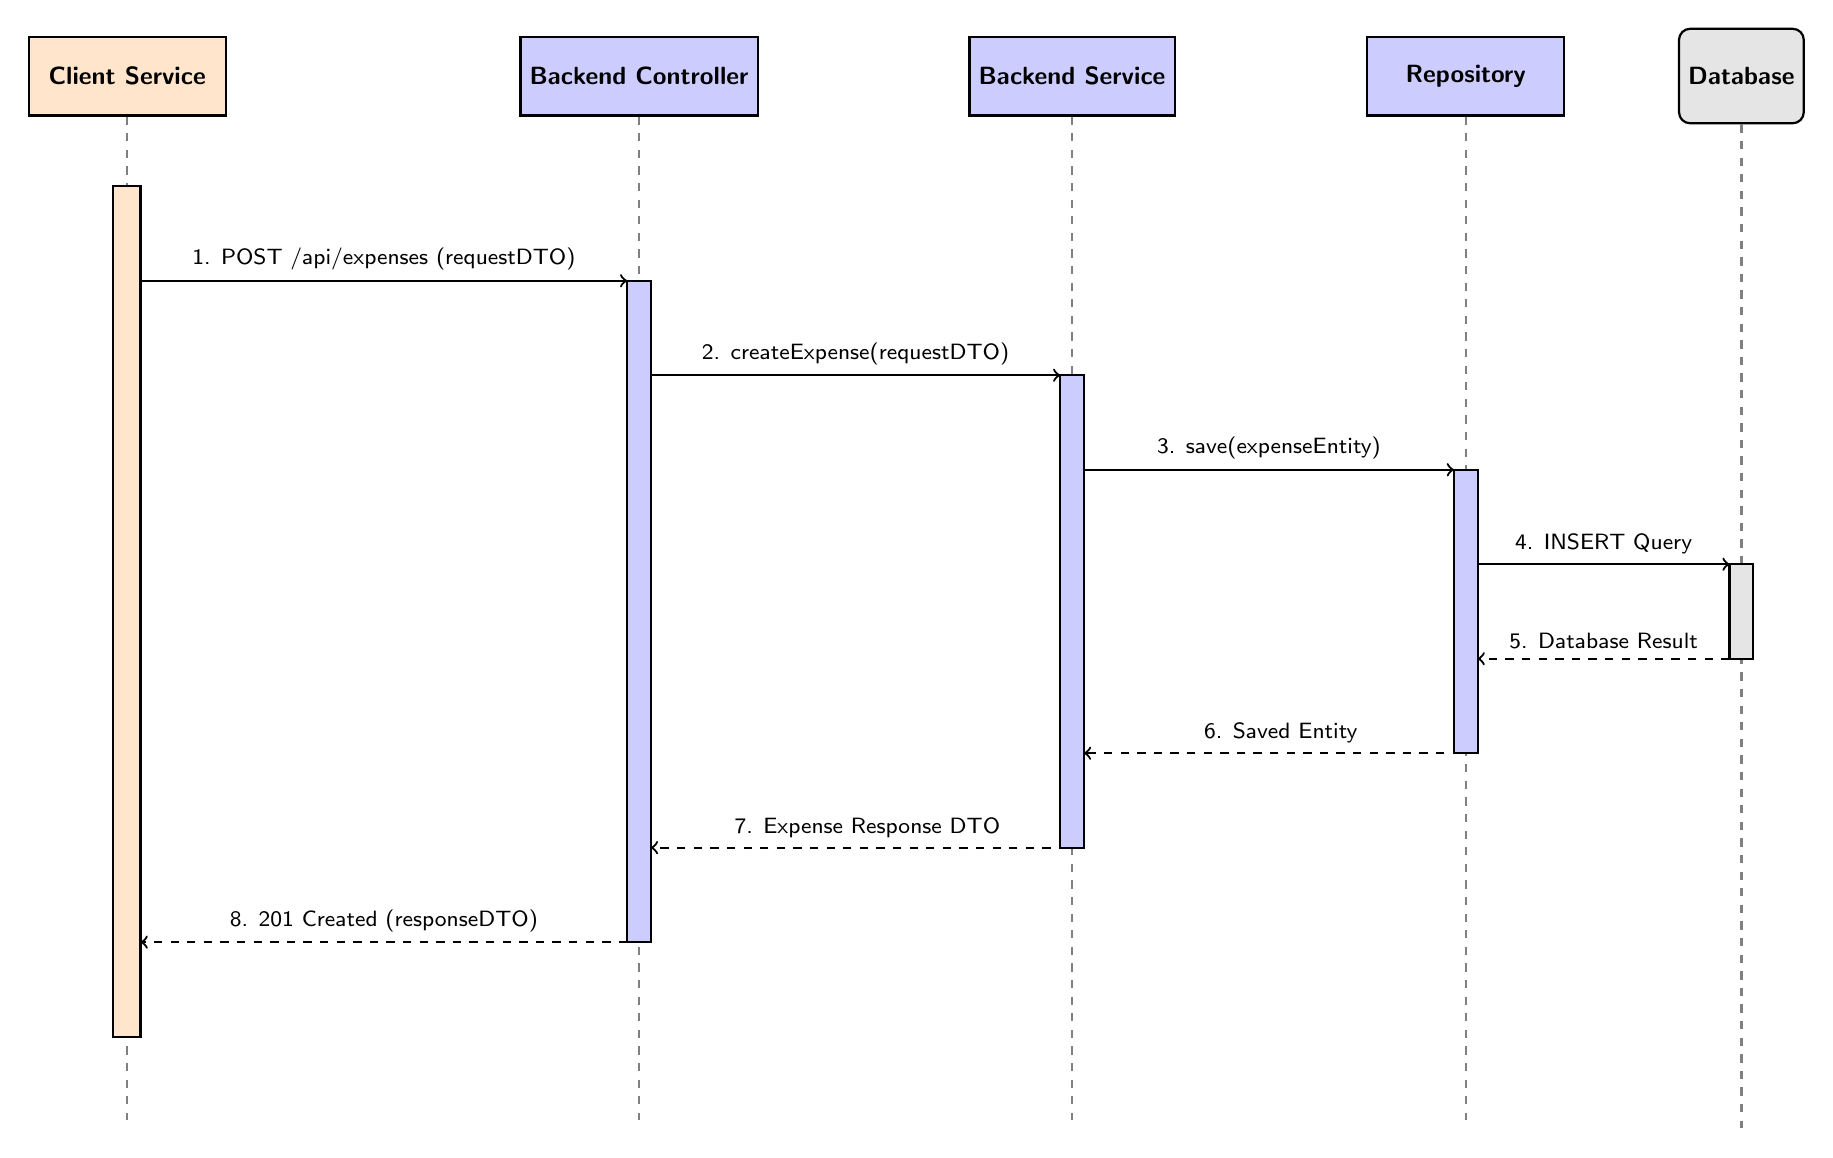
\begin{tikzpicture}[
    lifeline/.style={thick, dashed, draw=gray},
    box/.style={draw=black, thick, fill=blue!5, minimum width=2.5cm, minimum height=1cm, font=\sffamily\small\bfseries, align=center},
    dbbox/.style={draw=black, thick, rounded corners, minimum height=1.2cm, minimum width=1.5cm, fill=yellow!10, align=center, font=\sffamily\small\bfseries},
    msg/.style={->, thick, font=\footnotesize\sffamily},
    return/.style={->, dashed, thick, font=\footnotesize\sffamily}
]

% Nodes
\node[box, fill=orange!20] (client) at (-0.5, 1.6) {Client Service};
\node[box, fill=blue!20] (controller) at (6, 1.6) {Backend Controller};
\node[box, fill=blue!20] (service) at (11.5, 1.6) {Backend Service};
\node[box, fill=blue!20] (repository) at (16.5, 1.6) {Repository};
\node[dbbox, fill=gray!20] (db) at (20, 1.6) {Database};

% Lifelines
\draw[lifeline] (client.south) -- +(0, -12.75);
\draw[lifeline] (controller.south) -- +(0, -12.75);
\draw[lifeline] (service.south) -- +(0, -12.75);
\draw[lifeline] (repository.south) -- +(0, -12.75);
\draw[lifeline] (db.south) -- +(0, -12.75);

% UML Activation Boxes
\draw[fill=orange!20, draw=black, thick] (-0.68, 0.2) rectangle (-0.33, -10.6);   % Client
\draw[fill=blue!20, draw=black, thick] (5.85, -1) rectangle (6.15, -9.4);    % Controller
\draw[fill=blue!20, draw=black, thick] (11.35, -2.2) rectangle (11.65, -8.2);  % Service
\draw[fill=blue!20, draw=black, thick] (16.35, -3.4) rectangle (16.65, -7.0); % Repository
\draw[fill=gray!20, draw=black, thick] (19.85, -4.6) rectangle (20.15, -5.8); % DB

% Messages
\draw[msg] (-0.33, -1) -- node[above] {1. POST /api/expenses (requestDTO)} (5.85, -1);
\draw[msg] (6.15, -2.2) -- node[above] {2. createExpense(requestDTO)} (11.35, -2.2);
\draw[msg] (11.65, -3.4) -- node[above] {3. save(expenseEntity)} (16.35, -3.4);
\draw[msg] (16.65, -4.6) -- node[above] {4. INSERT Query} (19.85, -4.6);

\draw[return] (19.85, -5.8) -- node[above] {5. Database Result} (16.65, -5.8);
\draw[return] (16.65, -7.0) -- node[above] {6. Saved Entity} (11.65, -7.0);
\draw[return] (11.65, -8.2) -- node[above] {7. Expense Response DTO} (6.15, -8.2);
\draw[return] (5.85, -9.4) -- node[above] {8. 201 Created (responseDTO)} (-0.33, -9.4);

\end{tikzpicture}}%
\caption{User request flow: Adding an Expense}
\end{figure}